\documentclass{article}
\usepackage[utf8]{inputenc}
\usepackage[a4paper, margin=2.5cm]{geometry}
\usepackage{graphicx} 
\usepackage{natbib}
\usepackage[french]{babel}

%\usepackage[default,scale=0.95]{opensans}
\usepackage[T1]{fontenc}
\usepackage{amssymb} %math
\usepackage{amsmath}
\usepackage{amsthm}
\usepackage{systeme}
\usepackage{bbm}
\usepackage{media9}
\usepackage{makecell}
\usepackage{url}
\usepackage{minted}
\usepackage{xcolor}
\usepackage{wrapfig}
\usepackage{csquotes}
\usepackage{subcaption}
\usepackage{float}
\usepackage{dirtree}

% \usepackage{lineno}
% \linenumbers

\usepackage{hyperref}
\hypersetup{
    % colorlinks=true,
    % linkcolor=blue,
    % filecolor=magenta,      
    % urlcolor=cyan,
    pdftitle={Projet RITAL},
    %pdfpagemode=FullScreen,
    }
\urlstyle{same} %\href{url}{Text}

\renewcommand{\baselinestretch}{1.5}
\graphicspath{{./src/}}

\begin{document}

\begin{titlepage}
    \begin{center}
        \vspace*{1cm}

        \Huge
        \textbf{ML - Projet}

        %\vspace{0.5cm}
        \LARGE
        Réseau de neurones from scratch

        %\vspace{1.5cm}
        \Large
        Charles \textsc{Vin}, Aymeric \textsc{Delefosse}

        \vfill
        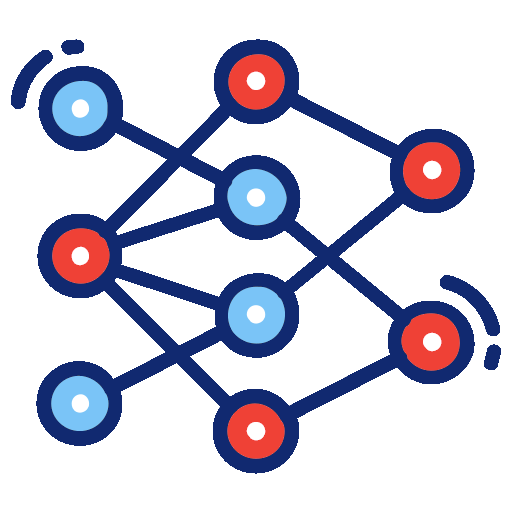
\includegraphics[width=.5\textwidth]{neural-network.png}    
        \vfill

        \large
        DAC | 2022-2023 \hfill 
        
\includegraphics[width=0.30\textwidth]{logo.png}
        \hfill
        
        
    \end{center}
\end{titlepage}

\tableofcontents
\newpage

\section{Introduction}

\section{Implémentation}

Le code est disponible sur \href{https://github.com/dataymeric/NeuralNetworksDIY}{ce dépôt GitHub}.

La bibliothèque est organisée de la manière suivante :


\section{Expérimentation}

Dans le but de mettre notre bibliothèque à l'épreuve, nous avons entrepris une série d'expérimentations en utilisant diverses architectures sur deux types de données distincts. Le premier ensemble de données était constitué de jeux aléatoires de données gaussiennes, présentant des caractéristiques linéairement séparables ou non, tels que le XOR ou le jeu d'échecs. Le second ensemble de données concernait la classification d'images sur le Fashion MNIST.

\subsection{Classification}

\subsubsection{Impact de l'initialisation des paramètres}

Nous avons très vite constaté le rôle et l'impact de l'initialisation des paramètres sur les performances des réseaux de neurones. Cette initialisation peut paraître anodine à première vue mais joue un rôle crucial sur la performance et la significativité du modèle. \\
Une initialisation inadéquate peut entraîner des problèmes tels que la saturation des neurones, la divergence de l'apprentissage ou la stagnation dans des minima locaux. Une initialisation judicieuse peut quant à elle favoriser une convergence plus rapide et une meilleure généralisation des données. \\
Ainsi, l'optimisation des poids et des biais à l'initialisation constitue une étape cruciale dans la conception et l'entraînement des réseaux de neurones. Cette initialisation peut se faire en prenant en compte les spécificités de l'architecture et de la fonction d'activation.

Ainsi, pour les modules utilisant des paramètres (linéaire et convolution), il est possible d'initialiser les poids et biais de huit manières différentes :

\begin{itemize}
    \item Initialisation normale : les paramètres sont initialisés selon une loi normale centrée réduite : $ W \sim \mathcal{N}(0, 1) $ ;
    \item Initialisation uniforme : les paramètres sont initialisés selon une loi uniforme : $ W \sim \mathcal{U}(0, 1) $ ;
    \item Initialisation à 1 : très simpliste, tous les paramètres sont initialisés à 1 ;
    \item Initialisation à 0 : très simpliste, tous les paramètres sont initialisés à 0 ;
    \item Initialisation de Xavier (ou de Glorot) : cette méthode, développée par Xavier Glorot et Yoshua Bengio, ajuste les poids de manière à maintenir une variance constante tout au long du réseau, en fonction du nombre d'entrées et de sorties de chaque couche. Cela favorise une propagation efficace du signal. Il est possible d'initialiser selon une loi normale ou une loi uniforme, où $ \text{input} $ représente la taille de l'entrée dans le cadre d'un module linéaire, le nombre de canaux d'entrée dans le cadre d'une convolution et $ \text{output} $ représente la taille de la sortie dans le cadre d'un module linéaire, le nombre de canaux en sortie (le nombre de \textit{feature maps}) dans le cadre d'une convolution.
    \begin{itemize}
        \item Loi normale : $ W \sim \mathcal{N}(0, \sqrt[]{\frac{2}{\text{input} + \text{output}}}) $ ;
        \item Loi uniforme : $ W \sim \mathcal{U}(- \sqrt[]{\frac{6}{\text{input} + \text{output}}}, \sqrt[]{\frac{6}{\text{input} + \text{output}}}) $.
    \end{itemize}
    \item Initialisation de He (ou de Kaiming) : Cette méthode, développée par Kaiming He et al., est similaire à l'initialisation de Xavier, mais elle prend en compte la variance spécifique des fonctions d'activation asymétriques, telles que la fonction ReLU. Elle permet une initialisation adaptée aux architectures utilisant ces fonctions d'activation. 
    \begin{itemize}
        \item Loi normale : $ W \sim \mathcal{N}(0, \sqrt[]{\frac{2}{\text{input}}}) $ ;
        \item Loi uniforme : $ W \sim \mathcal{U}(- \sqrt[]{\frac{6}{\text{input}}}, \sqrt[]{\frac{6}{\text{input}}}) $.
    \end{itemize}
\end{itemize}

\textbf{Note} : pour le module linéaire, les biais sont initialisés par défaut tandis que pour la convolution, les biais sont désactivés par défaut (sauf indication contraire).

\begin{figure}[htbp]
    \centering
    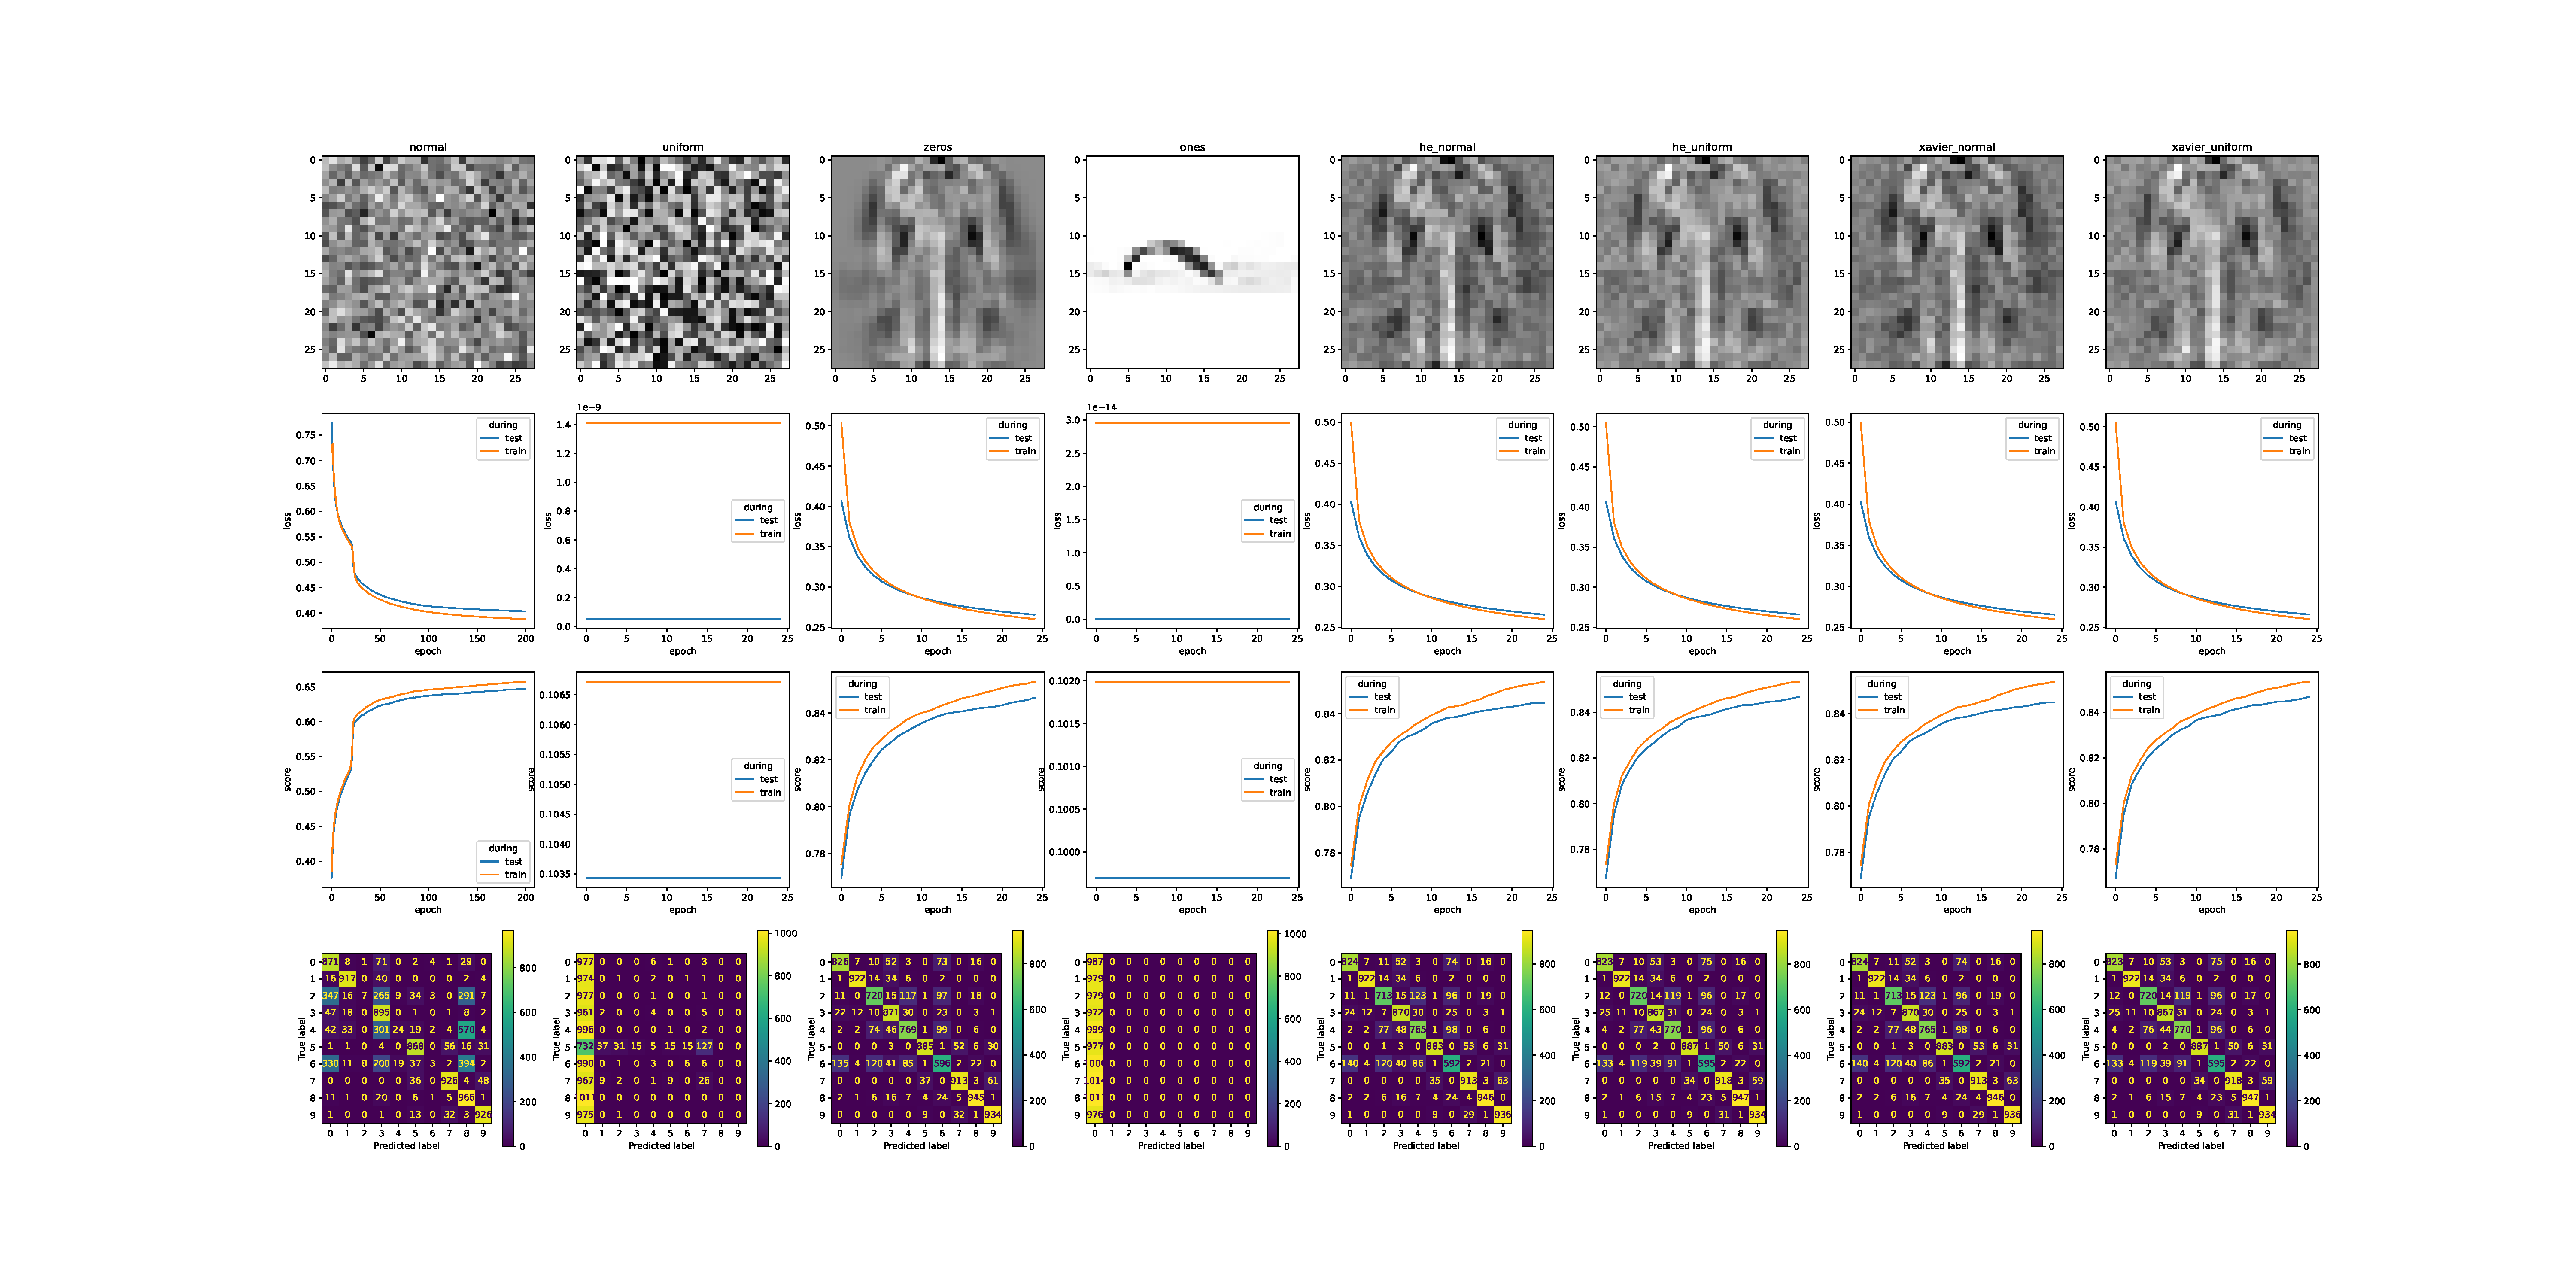
\includegraphics[width=\textwidth]{init_type.pdf}
    \caption{Représentation des paramètres, d'une matrice de confusion, de l'évolution du coût et du score par époque en fonction de l'initialisation des paramètres}
    \label{fig:initparam}
\end{figure}

Pour déterminer en pratique l'effet de l'initialisation des paramètres, nous avons mis en place un réseau très simple qui classifie le jeu de données \textit{fashion-mnist}. Celui-ci est composé d'une couche linéaire prenant en entrée l'image entière et classifiant sur dix neurones en sortie. On représentera par la suite les réseaux sous la forme suivante \texttt{Linear(784, 10) $ \rightarrow $ Sigmoid()}.f

La figure \ref{fig:initparam} représente les résultats de cette expérimentation. On constate des difficultés d'apprentissage sur certaine initialisation. L'initialisation normal tombe dans un minimum local (200 époques). Les initialisations uniforme et à 1 font exploser le gradient, empechant tout apprentissage. 

Cette expérience a montrer l'impact important que peux avoir l'initialisation des poids. L'initialisation normale pourrait certainement être fixer en utilisant un autre optimiser, tel que Adam.

\subsubsection{Effet du taux d'apprentissage (\textit{learning rate})}

Le \textit{learning rate} est un hyperparamètre crucial dans l'entraînement des réseaux de neurones. Il contrôle la taille des pas que l'algorithme d'optimisation effectue lors de la mise à jour des poids du réseau pendant l'apprentissage. Un taux d'apprentissage adapté permet aux mises à jour de poids d'être suffisamment grandes pour converger rapidement vers un minimum, tout en évitant les oscillations et les divergences. Le but est donc de trouver un bon compromis entre la rapidité de convergence et la stabilité des résultats.

\begin{figure}[htbp]
    \centering
    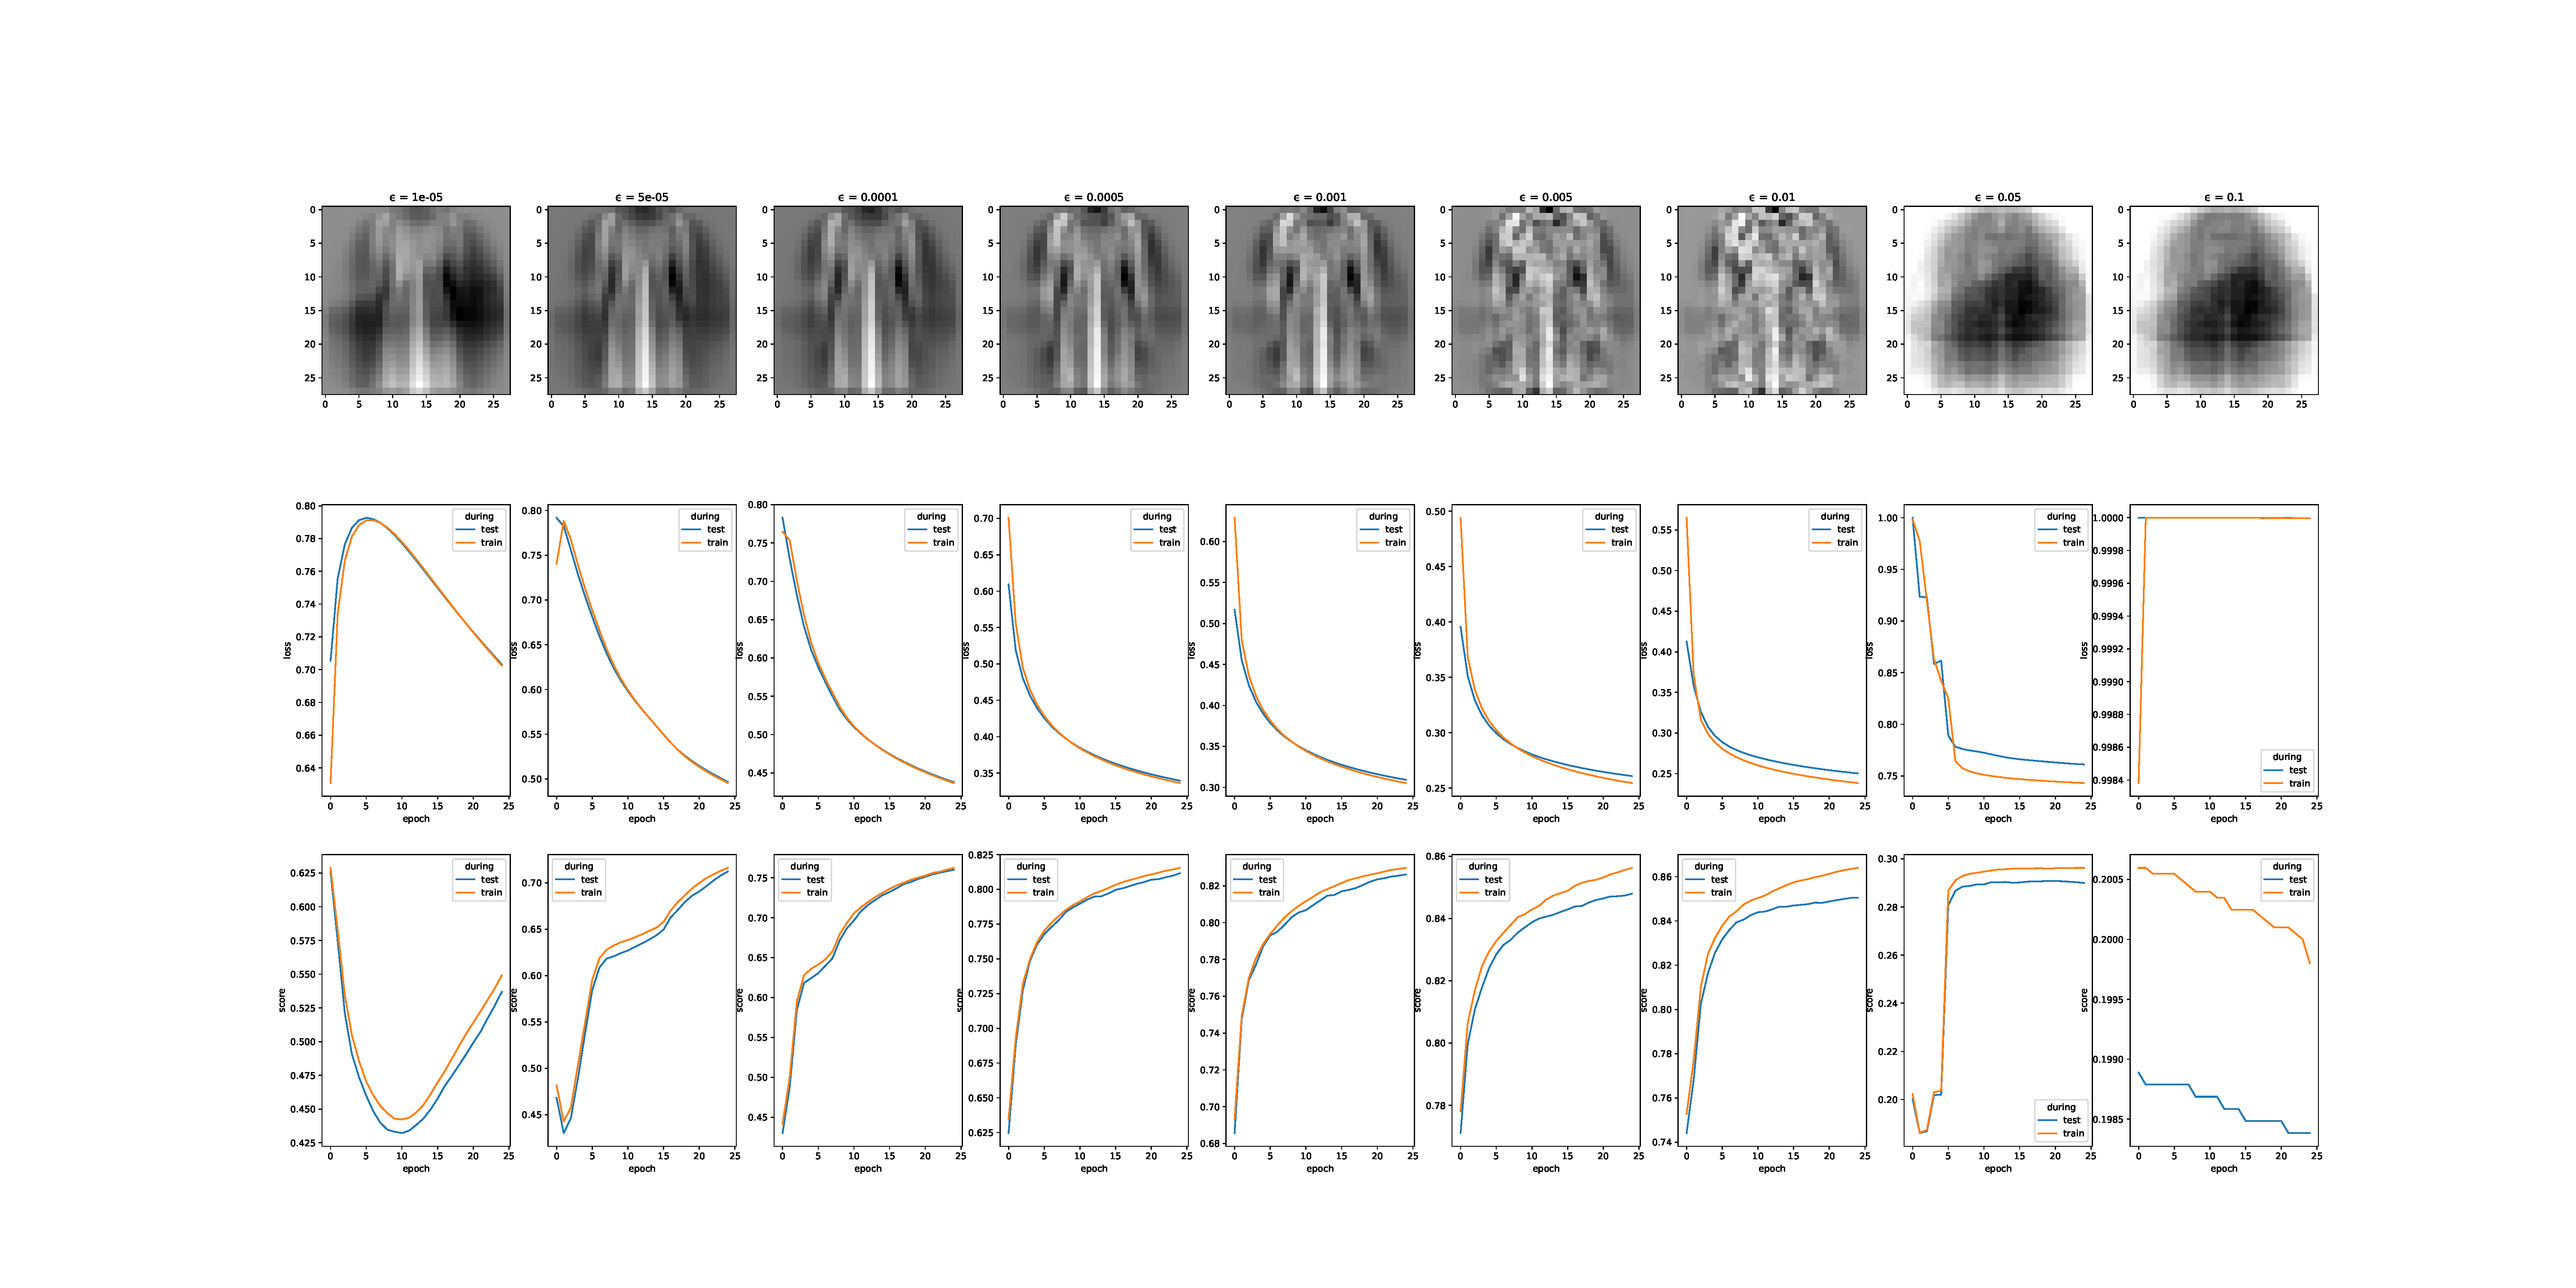
\includegraphics[width=\textwidth]{lr_effet.pdf}
    \caption{Représentation des paramètres, de l'évolution du coût et du score par époque en fonction du taux d'apprentissage $ \epsilon $ }
    \label{fig:effetlearningrate}
\end{figure}

Toujours avec le même réseau très simple, nous obtenons les résultats dans la figure \ref{fig:effetlearningrate}. 

Un \textit{learning rate} trop faible ralentit donc la convergence, et un nombre élevé d'itérations sera nécessaire pour atteindre une performance obtenue avec un taux d'apprentissage plus élevé. Les ajustements apportés aux poids sont également plus lents et progressifs, au risque de rester coincer dans des minima locaux peu optimaux.

Un \textit{learning rate} trop élevé entraîne une divergence dans notre cas, les poids se mettent à jour trop brutalement entraînant une convergence vers un modèle sous-optimal.

\subsubsection{Effet des fonctions d'activation}

La fonction d'activation joue un rôle essentiel dans les réseaux de neurones : elle introduit une non-linéarité dans les activations du réseau, ce qui permet au modèle d'apprendre des représentations non linéaires complexes des données.

L'ajout d'une fonction d'activation non linéaire après un module linéaire, tel qu'une couche dense ou une convolution, permet d'introduire des interactions non linéaires entre les neurones et d'augmenter la capacité de représentation du modèle. Sans fonction d'activation, le réseau de neurones se réduirait simplement à une combinaison linéaire des entrées, limitant ainsi sa capacité à modéliser des relations complexes.

Différentes fonctions d'activation peuvent être utilisées en fonction du problème et des caractéristiques des données. Par exemple :

\begin{itemize}
    \item La fonction tangente hyperbolique qui comprime les sorties dans $ [-1, 1] $ ;
    \item La fonction sigmoïde qui comprime les sorties entre 0 et 1 ;
    \item La fonction sigmoïde "stable" qui a été implémenté dans l'optique d'éviter des potentiels explosions de gradient et instabilités numériques ;
    \item La fonction softmax pour transformer les données en une distribution de probabilités ;
    \item La fonction log-softmax afin d'éviter des instabilités numériques ;
    \item La fonction ReLU ;
    \item La fonction LeakyReLU afin d'éviter du \textit{gradient vanishing} et empêcher la rétropropagation du gradient ;
    \item La fonction SoftPlus qui est une autre approximation de la fonction ReLU.
\end{itemize}

On pourrait, rajouter encore d'autres fonctions d'activation, telles que la fonction identité, une identité courbée, une sinusoïde, un sinus cardinal, une fonction gaussienne.

Le choix de la fonction d'activation dépend du problème à résoudre, des caractéristiques des données et de l'architecture du réseau. Chaque fonction d'activation a des propriétés différentes et peut être plus adaptée à certains types de problèmes ou à certaines architectures.

\begin{figure}[htbp]
    \centering
    % 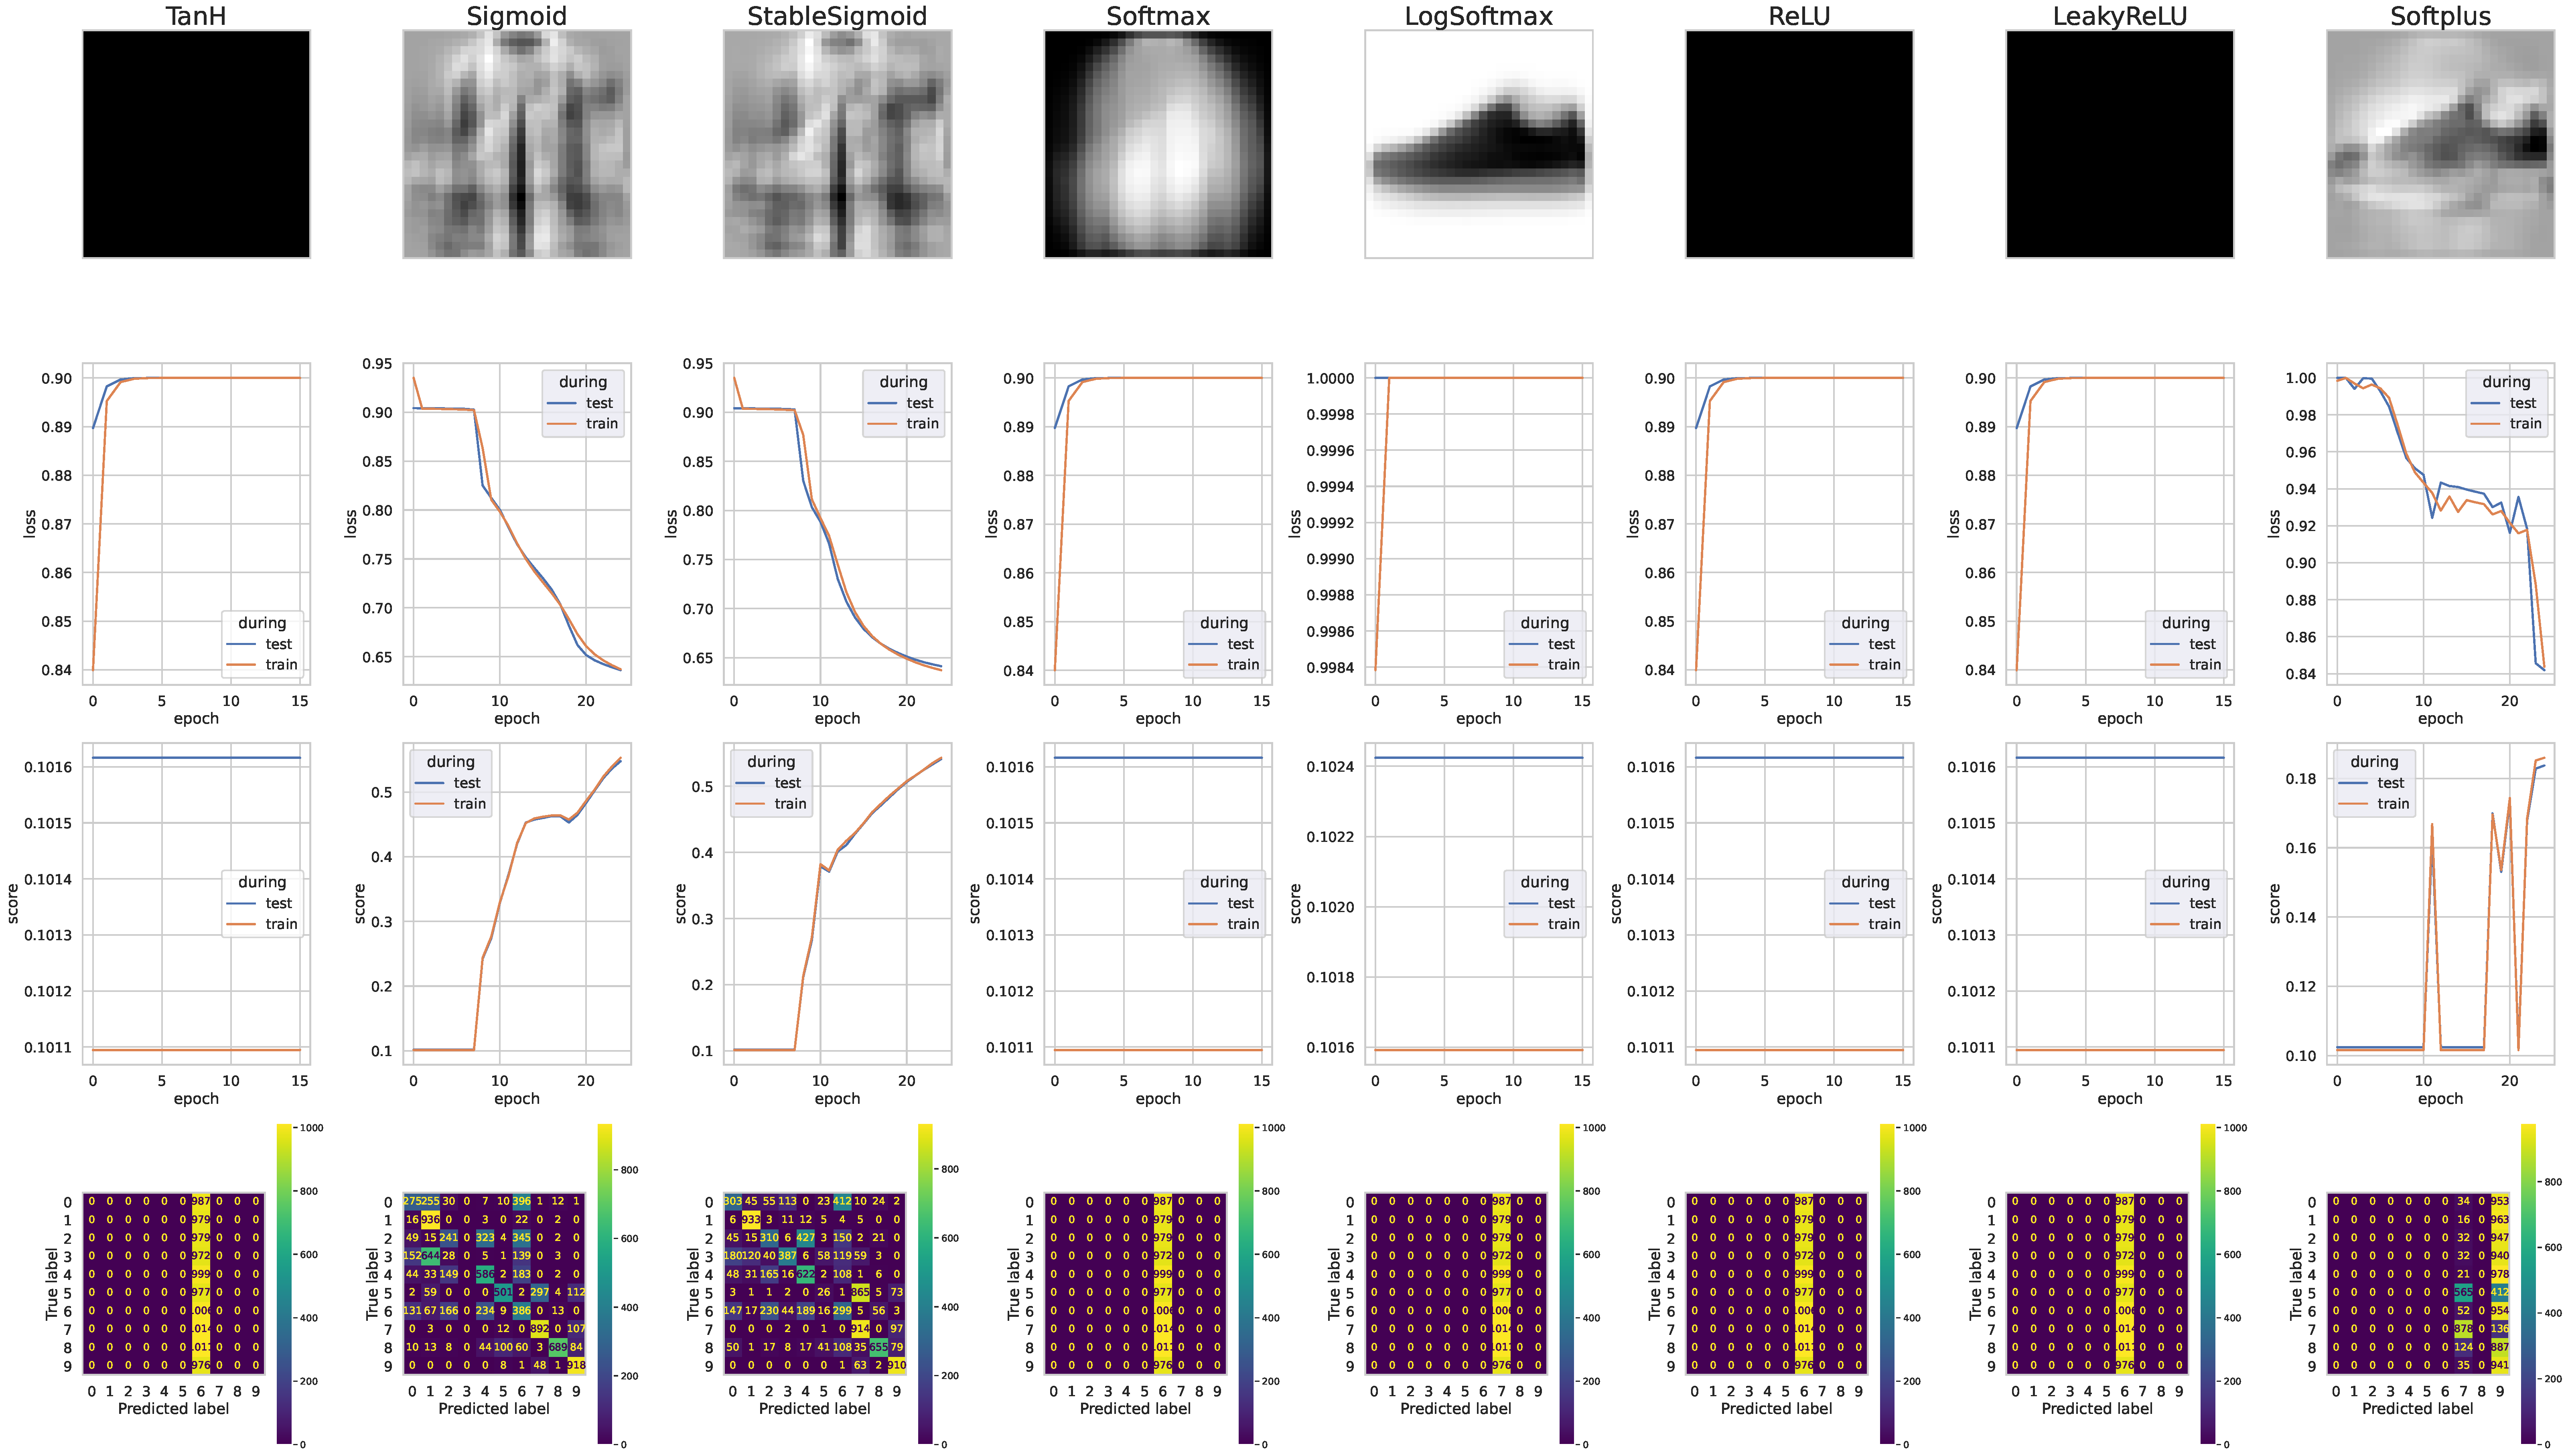
\includegraphics[width=\textwidth]{activation_func.pdf}
    \caption{Représentation des paramètres, de l'évolution du coût et du score par époque en fonction du taux d'apprentissage $ \epsilon $ }
    \label{fig:activationfunc}
\end{figure}

\subsection{Encoder-Decoder sans convolutions}
\subsubsection{Reconstruction}
\subsubsection{Débruitage}

\subsection{Encoder-Decoder avec convolution}
\subsubsection{Reconstruction}
\subsubsection{Débruitage}

\subsection{Transfert de style}


\end{document}